	\chapter{Einf\"uhrung in OpenCL}
	\textit{Open Computing Language} (OpenCL) ist eine freie open-source Programmierschnittstelle für paralleles Rechnen, die von Apple im Jahr 2009 entwickelt wurde. Heute liegt diese in Version 2.2 vor und wird von der Khronos Gruppe entwickelt, der sich mittlerweile über 200 Firmen angeschlossen haben. Das Ziel hinter dem Projekt ist, eine low-level Programmiersprache und Schnittstelle zu schaffen, mit denen sich maximal inhomogene Parallelrechner (CPUs, GPUs, Grafikchips, FPGAs, Beschleuniger, ...) programmieren lassen und dabei Plattformunabhängigkeit gewährleisten. Ein Gerät benötigt dafür eine Hardwareimplementierung und der Hersteller muss eine OpenCL Implementierung in Software bereitstellen (z.B. AMD, Intel, ...). Im Nvidia Toolkit ist eine OpenCL Installation enthalten, in Hardware aber nur für Version 1.2 implementiert. C- und C++-\Glspl{API} sind gewöhnliche Librarys, die unter Linux über die Paketquellen installiert werden können.
	
	Die Khronos Gruppe entwickelt ebenfalls die Grafikbibliothek OpenGL und Nachfolger Vulkan, für die ähnliche Prinzipien gelten. 
	 
	    \section{Begriffe}
	    Obwohl Nvidia ebenfalls Teil der Khronos Gruppe ist, haben sich in der Fachsprache hier andere Begriffe etabliert. Tabelle \ref{tab4:begriffe} zeigt typische OpenCL Begriffe und ihre Entsprechung in CUDA.
	    	\begin{table}[h]
	    		\centering
	    		\begin{tabular}{ll}
	    			\toprule 
	    			\textbf{OpenCL} & \textbf{CUDA} \\ \hline
	    			Workitem & Thread \\
	    			Workgroup & Block \\ \hline
	    			Global Memory & Global Memory \\
	    			Constant Memory & Constant Memory \\
	    			Local Memory & Shared Memory \\
	    			Private Memory & Local Memory \\ \hline
	    			Platform & \textit{keine} \\
	    			Device & Device \\
	    			Context & \textit{keine} \\
	    			Command Queue & Stream \\
	    			Kernel & Kernel \\
	    			Event & Event \\ \hline
	    			Global Work Size & Grid Size \\
	    			Local Work Size & Block Size \\
	    			Work Dimension & Grid/Block Dimension \\
	    			\bottomrule
	    		\end{tabular}
	    		\caption{Typische OpenCL Begriffe und ihre Entsprechung in CUDA}
	    		\label{tab4:begriffe}
	    	\end{table}
	    	Technisch gesehen sind sich AMD und Nvidia Grafikkarten ähnlich. Allerdings nennt AMD die \Glspl{Warp} \Glspl{Wavefront} und deren Größe ist abhängig vom Chip entweder 32 oder 64. Demnach sollte bei entsprechender Größe die Local Work Size, also die Größe einer \Gls{Workgroup}, ein Vielfaches von 32 oder 64 sein. 
	    	
	    	Diese Einführung beschränkt sich auf das Programmieren von GPUs. Die dafür verwendeten Befehle sind CUDA sehr ähnlich und tragen lediglich andere Namen. Tabelle \ref{tab4:begriffe} zeigt eine Auflistung der wichtigsten.
	    	
	    	\begin{table}[h]
	    		\centering
	    		\scalebox{0.9}{%
	    		\begin{tabular}{ll}\toprule
	    			\textbf{OpenCL} & \textbf{CUDA} \\ \midrule
					\li`__kernel`, \li`kernel` & \li`__global__` \\
					\li`__constant`, \li`constant` & \li`__constant__` \\
					\li`__global`, \li`global` & \textit{automatisch} \\
					\li`__private`, \li`private` & \textit{automatisch} \\
					\li`__local`, \li`local` & \li`__shared__` \\
\hline					
					\li`get_global_id(0)` & \li`blockIdx.x*blockdim.x + threadIdx.x` \\
					\li`get_global_id(1)` & \li`blockIdx.y*blockdim.y + threadIdx.y` \\
					\li`get_global_id(2)` & \li`blockIdx.z*blockdim.z + threadIdx.z` \\
\hline					
					\li`get_local_id(0)` & \li`threadIdx.x` \\
					\li`get_local_id(1)` & \li`threadIdx.y` \\
					\li`get_local_id(2)` & \li`threadIdx.z` \\
\hline					
					\li`get_local_size(0)` & \li`blockdim.x` \\
					\li`get_local_size(1)` & \li`blockdim.y` \\
					\li`get_local_size(2)` & \li`blockdim.z` \\
\hline																				
					\li`get_global_size(0)` & \li`griddim.x` \\
					\li`get_global_size(1)` & \li`griddim.y` \\
					\li`get_global_size(2)` & \li`griddim.z` \\
					
					\li`clCreateBuffer(...)` & \li`cudaMalloc(...)` \\
					\li`clEnqueueWriteBuffer(...)` & \li`cudaMemcpy(Async)(..., cudaMemcpyHostToDevice)` \\
					\li`clEnqueueReadBuffer(...)` & \li`cudaMemcpy(Async)(..., cudaMemcpyDeviceToHost)`  \\
					\li`clEnqueueCopyBuffer(...)` & \li`cudaMemcpy(Async)(..., cudaMemcpyDeviceToDevice)`  \\
					\li`clEnqueueNDRangeKernel(..., <Kernel>, ...)`, \li`clSetKernelArg(...)` & \li`<kernelcall><<<...>>>(...)` \\
\hline
					\li`barrier(CLK_LOCAL_MEM_FENCE)` & \li`__syncthreads()` \\
					\li`barrier(CLK_GLOBAL_MEM_FENCE)` & \li`__syncthreads()` \\
					\li`barrier(CLK_IMAGE_MEM_FENCE)`\footnote{wurde in späteren Versionen in \li`work_group_barrier(...)` umbenannt} & \textit{keine} \\ \bottomrule
	    		\end{tabular}}
	    		\caption{Typische OpenCL Befehle/Keywords und ihre Entsprechung in CUDA}
	    		\label{tab4:befehle}
	    	\end{table}
	    	
	    	Für die Nvidia Produktlinien Geforce, Quadro und Tesla existieren bei AMD die Entsprechungen Radeon, Radeon Pro und Radeon Instinct. 
	    	
		\section{Programmiermodell}
		Im Gegensatz zu CUDA fordert OpenCL eine strikte Trennung von Host- und Devicecode in verschiedenen Dateien. Das Hostprogramm wird mittels der OpenCL C-\Gls{API} programmiert (oder C++ Wrapper), bei der es sich um eine gewöhnliche C-Library handelt. Dieses Hostprogramm wird mit einem beliebigen C- oder C++-Compiler übersetzt und unterstützt damit auch die modernsten Features beider Programmiersprachen.
		
		Die Deviceprogramme liegen in Form von \Gls{Kernel} in einer oder mehrerer seperater Dateien vor, die als String vom Hostprogramm eingelesen werden. Dies hat den Vorteil, dass zu Compilezeit der Inhalt des Programms nicht bekannt sein muss und damit auch nicht verändert wird. Erst zur Laufzeit wird unsichtbar für den Nutzer der OpenCL Compiler gerufen und das OpenCL Programm kompiliert und ausgeführt (Just-In-Time Compiler, JIT). Bei einer Änderung eines \Glspl{Kernel} muss das Hostprogramm also nicht noch ein weiteres Mal kompiliert werden.
		
		Devicecode wird in der eigentlichen Programmiersprache OpenCL C geschrieben, die sich im Wesentlichen an C99 orientiert. Teilweise wurde auch C++ unter dem Namen OpenCL C++ implementiert (siehe \ref{OCLC++}). Es folgt eine Auflistung der wichtigsten Einschränkungen:
		\begin{itemize}
	        	\item keine C99-Standard Header, Ersatz ist der Vorrat von built-in-Funktionen.
        		\item Kernel-Zeigerargumente müssen mit \li`__global`, \li`__constant`, oder \li`__local` qualifiziert werden.  
		    \item nur \li`__constant`-Zeiger dürfen \li`__constant`-Zeigern zugewiesen werden.
        		\item keine Zeiger auf Funktionen.
		    \item keine Bitfelder.
        		\item keine VLAs (variable length arrays).
		    \item weder Makros noch Funktionen mit variabler Argumentzahl (außer \li`enqueue_kernel`).
        		\item keine auto und register Speicherklassen.
		    \item keine rekursiven Funktionen.
        		\item \Glspl{Kernel} sind immer Prozeduren mit \li`void`-Ergebnis.
		    \item keine \Gls{Kernel}-Argumente mit den Typen \li`bool`, \li`half`, \li`size_t`, \li`ptrdiff_t`, \li`intptr_t`, \li`uintptr_t`, sowie Strukturen und Unions mit einer dieser Komponenten.
        		\item keine Arithmetik für \li`half`, nur Speicherformat.
		    \item irreduzible Anweisungsgruppen (z.B. Sprünge in Schleifen) sind implementation-defined.
        		\item \li`const`, \li`restrict` und \li`volatile` sind erlaubt, aber für Images verboten.
		    \item \li`event_t` darf kein \Gls{Kernel}-Argument sein.
        		\item  \li`event_t` darf nicht zusammen mit \li`__local`, \li`__constant` and \li`__global` verwendet werden.
		\end{itemize}
		
            \subsection{Plattformen}
            Da mehrere verschiedene Implementierungen von OpenCL existieren, muss zunächst eine \Gls{Platform} ausgewählt werden. Die Khronos Gruppe aktualisiert stetig die Liste aller Plattformen: \url{https://www.khronos.org/conformance/adopters/conformant-products/opencl}
            \begin{lstlisting}[caption=Plattformabfrage]
        cl_platform_id platform_id = NULL;
        uint ret_num_platforms;
        clGetPlatformIDs(1, &platform_id, &ret_num_platforms);
            \end{lstlisting}

			\li`platform_id` kann bei mehreren Plattformen ein Array von IDs sein. In diesem Fall muss im ersten Argument angegeben werden, nach wie vielen Plattformen gesucht werden soll.
			
			Die meisten \Gls{API} Aufrufe geben einen Fehlercode zurück, der in einer Tabelle nachgeschlagen werden kann: \url{https://streamhpc.com/blog/2013-04-28/opencl-error-codes/}
			
			Im Folgenden werden nur die OpenCL eigenen Datentypen verwendet (siehe \ref{makros}).
							
            \subsection{Devices}
            Jede \Gls{Platform} stellt OpenCL für ein oder auch mehrere Geräte zur Verfügung. Im nächsten Schritt müssen also die entsprechenden Devices den gefundenen \Glspl{Platform} zugeordnet werden.		
            \begin{lstlisting}[caption=Deviceabfrage]
        cl_device_id device_id = NULL;	
        uint ret_num_devices;
        clGetDeviceIDs(platform_id, CL_DEVICE_TYPE_DEFAULT, 1, 
            &device_id, &ret_num_devices);
            \end{lstlisting}
			
            Auch hier kann \li`device_id` ein Vektor sein. Die zweite Eingabe bezeichnet als Bitfeld die Device Typen, die abgefragt werden sollen. Mehrere Typen können mit dem Operator | abgetrennt werden. Für den Typ des Geräts existieren folgende Möglichkeiten:
						
            \begin{itemize}		
                \item \li`CL_DEVICE_TYPE_CPU`	
                \item \li`CL_DEVICE_TYPE_GPU`		
                \item \li`CL_DEVICE_TYPE_ACCELERATOR`		
                \item \li`CL_DEVICE_TYPE_DEFAULT`			
                \item \li`CL_DEVICE_TYPE_ALL`
            \end{itemize}
				
			\subsection{Kontexte}
			Ein \Gls{Kontext} ist ein \Gls{Handle} für das OpenCL Programm. Dieser beinhaltet Speicherobjekte, Programme und Command Queues. Folglich müssen diese also einem neu erstellten \Gls{Kontext} zugeordnet werden. Abbildung \ref{4:class} zeigt die Zusammenhänge sämtlicher OpenCL Klassen \autocite{oclRC} basierend auf der Unified Modelling Language (UML). \autocite{uml}
			\begin{lstlisting}[caption=Kontexte]
			cl_int ret;
			cl_context context = clCreateContext(NULL, 1, &device_id, 
				NULL, NULL, &ret);	
			\end{lstlisting}
			
			Sollte eine Funktion über einen eigenen Rückgabewert verfügen, so ist das letzte Argument üblicherweise ein Pointer auf einen Fehlercode.
			\begin{figure}[h]
				\centering
				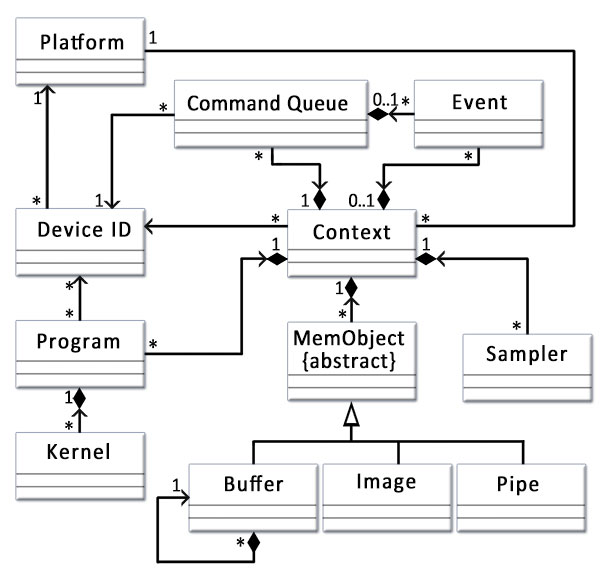
\includegraphics[width=0.7\textwidth]{chapter4/pictures/class.png}
				\caption{Zusammenhänge sämtlicher OpenCL Klassen}
				\label{4:class}
			\end{figure}				
				
			\subsection{Programme}
			Als nächstes muss das OpenCL Programm als String gelesen, zur Laufzeit kompiliert und dem Kontext hinzugefügt werden. 
			\begin{lstlisting}[caption=OpenCL Programm]
			FILE *fp;
			char *source_str;
			size_t source_size;
			fp = fopen("cl_vecadd.cl", "r");
			if(!fp)
			{
				fprintf(stderr, "Failed to load the kernel!\n");
				exit(1);
			}
			fseek(fp, 0, SEEK_END);
			size_t s = ftell(fp);
			fseek(fp, 0, SEEK_SET); 
			source_str = (char*)malloc(s);
			source_size = fread(source_str, 1, s, fp);
			fclose(fp);
			
			cl_program program = clCreateProgramWithSource(context, 1, 
				(const char **)&source_str, (const size_t *)&source_size, &ret);
			\end{lstlisting}
			
			Mittels \li`clBuildProgram(program, 1, &device_id, "-D name=definition -I dir", NULL, NULL)` lassen sich ähnlich dem C-Compiler dem OpenCl Compiler zusätliche Informationen mitgeben (siehe auch \url{https://www.khronos.org/registry/OpenCL/sdk/1.0/docs/man/xhtml/clBuildProgram.html}). 
			
			Ebenso muss man hier eine Liste der Devices übergeben, für die der Code kompiliert werden soll. So lässt sich der Include-Pfad erweitern. Außerdem können mit \li`-D` Makros gesetzt werden. Eine Auflistung voreingestellter Makros findet sich in Kapitel \ref{makros}.
			
			Das vorletzte Argument kann einen Pointer auf eine Funktion enthalten, die nach erfolgreichem Kompilieren ausgeführt werden soll (Callback). Das letzte Argument kann die Argumente dieser Funktion beinhalten.
			
			Da an dieser Stelle erst das eigentliche OpenCL Programm kompiliert wird, muss nun der Output des OpenCL Compilers abgefragt werden.
					
			\begin{lstlisting}[caption=Fehlerabfrage OpenCL Compiler]
			if(ret != 0){
				size_t sz; char * bf;

				clGetProgramBuildInfo(program, device_id, CL_PROGRAM_BUILD_STATUS, 
					0, NULL, &sz);
				bf = (char*)malloc((sz+1) * sizeof(char));
				if(bf)
				{
					clGetProgramBuildInfo(program, device_id, CL_PROGRAM_BUILD_STATUS, 
						sz+1, bf, NULL);
					bf[sz] = 0;
					fprintf(stderr, "\n%s\n", bf);
					free(bf);
				}

				clGetProgramBuildInfo(program, device_id, CL_PROGRAM_BUILD_OPTIONS, 
					0, NULL, &sz);
				bf = (char*)malloc((sz+1) * sizeof(char));
				if(bf)
				{
					clGetProgramBuildInfo(program, device_id, CL_PROGRAM_BUILD_OPTIONS, 
						sz+1, bf, NULL);
					bf[sz] = 0;
					fprintf(stderr, "\n%s\n", bf);
					free(bf);
				}
				
				clGetProgramBuildInfo(program, device_id, CL_PROGRAM_BUILD_LOG, 
					0, NULL, &sz);
				bf = (char*)malloc((sz+1) * sizeof(char));
				if(bf)
				{
					clGetProgramBuildInfo(program, device_id, CL_PROGRAM_BUILD_LOG, 
						sz+1, bf, NULL);
					bf[sz] = 0;
					fprintf(stderr, "\n%s\n", bf);
					free(bf);
				} }
			\end{lstlisting}
			
			\newpage
			
			\subsection{Kernel}
			Danach kann das eigentliche \Gls{Kernel} erstellt werden. Dazu muss der Name der Funktion als String übergeben werden. Das Programmieren der Kernels funktioniert ähnlich wie in CUDA.			
            \begin{lstlisting}[caption=Kerneldefinition]
            __kernel void vecadd(__constant float *x, __constant float* y, 
                __global float *res, const int size)
            {
                int i = get_global_id(0);
                if(i < size)
                    res[i] = x[i] + y[i];
            }
            \end{lstlisting}
			
            \Glspl{Kernel} müssen mit dem Keyword \li`__kernel` deklariert. Der Rückgabewert ist immer \li`void`. Jedes Objekt liegt per Default im \gls{private Memory} des \Glspl{Workitem}. Arrays müssen also mit dem entsprechenden Keyword deklariert werden, \li`__global` für \gls{global Memory}, \li`__constant` für \gls{constant Memory} und \li`__local` für \gls{local Memory}. Die Unterstriche können weggelassen werden. 
			
			Eine zusätlich definierte Funktion kann vom \Gls{Kernel}, also vom Device aus, wie aus C gewohnt ausgeführt werden. 
			
			Für das \Gls{Kernel} müssen wie gewohnt Buffer erstellt und Speicher kopiert werden. Zudem müssen die Kernelargumente explizit gesetzt werden.
			\begin{lstlisting}[caption=Kernelaufruf]
			cl_mem d_x   = clCreateBuffer(context, CL_MEM_READ_ONLY, 
				size*sizeof(cl_float), NULL, &ret);
			cl_mem d_y   = clCreateBuffer(context, CL_MEM_READ_ONLY, 
				size*sizeof(cl_float), NULL, &ret);
			cl_mem d_res = clCreateBuffer(context, CL_MEM_WRITE_ONLY, 
				size*sizeof(cl_float), NULL, &ret);			
			cl_kernel kernel_vecadd = clCreateKernel(program, "vecadd", &ret);		
			size_t narg = 0;
			clSetKernelArg(kernel_vecadd, narg++, sizeof(cl_mem),  (void *)&d_x);
			clSetKernelArg(kernel_vecadd, narg++, sizeof(cl_mem),  (void *)&d_y);
			clSetKernelArg(kernel_vecadd, narg++, sizeof(cl_mem),  (void *)&d_res);
			clSetKernelArg(kernel_vecadd, narg++, sizeof(cl_uint), &size);
			\end{lstlisting}
			
			Ein Buffer kann in verschiedenen Modi erstellt werden (\ref{tab4:flags}).
			\begin{table}[h]
				\centering
				\begin{tabular}{ll}\toprule
				    \li`CL_MEM_READ_WRITE` & Zum Lesen und zum Schreiben (default) \\
    			        	\li`CL_MEM_WRITE_ONLY` & Das Objekt wird vom \Gls{Kernel} nicht gelesen \\	
	        			\li`CL_MEM_READ_ONLY`  & Das Objekt wird vom \Gls{Kernel} nicht geschrieben \\
        				\li`CL_MEM_USE_HOST_PTR` & Erstellt Speicher im Devicememory aus Hostarray.\\
				                             & Erstellen von verschiedenen Buffern aus dem selben Pointer\\
		        		                         & ist nicht definiert.\\
        				\li`CL_MEM_ALLOC_HOST_PTR` & Wie \li`CL_MEM_USE_HOST_PTR`, aber mit automatischer Allozierung \\
		        		\li`CL_MEM_COPY_HOST_PTR`  & Wie \li`CL_MEM_USE_HOST_PTR`, aber mit automatischer Kopie\\ \bottomrule
				\end{tabular}
				\caption{Buffermodi}
				\label{tab4:flags}
			\end{table}
			
			Das vorletzte Argument ist ein Pointer auf den Hostspeicher.
			
			Mehrere Flags können grundsätzlich über eine Abtrennung mit | gleichzeitig gesetzt werden. Mit der Angabe von \li`CL_TRUE` wird der Host blockiert (\li`CL_FALSE` entspricht also \li`cudaMemcpyAsync(...)`). Die Angabe danach gibt einen Offset auf der Speicheradresse an. Beim Erstellen des Buffers wird noch kein Speicher alloziert. Dies geschieht erst beim Kopieren oder falls \li`CL_MEM_COPY_HOST_PTR` gesetzt wurde.
							
			\subsection{Command Queues}
			Statt \Glspl{Stream} existieren in OpenCL \Glspl{Command Queue}. Jede Speicheranweisung (Kopieren, Lesen) muss in eine \Gls{Command Queue} eingereiht werden. Zum Schluss wird die Warteschlange mit dem \Gls{Kernel} ausgeführt und erzeugt dabei ein Event. Das Lesen des Speichers erfolgt, sobald dieses Event stattgefunden hat. Am Ende wird der Speicher freigegeben.
			
            \begin{lstlisting}[caption=Command Queues und Clean-Up]
        const cl_queue_properties  props = ...; 
        cl_command_queue command_queue = clCreateCommandQueueWithProperties(
            context, device_id, &props, &ret);

        clEnqueueWriteBuffer(command_queue, d_x, CL_TRUE, 0, 
            size*sizeof(cl_float), h_x, 0, NULL, NULL);	
        clEnqueueWriteBuffer(command_queue, d_y, CL_TRUE, 0,
            size*sizeof(cl_float), h_y, 0, NULL, NULL);			
				
        size_t global_item_size = ... //Zahl der Workitems gesamt
        size_t local_item_size = ... //Größe der Workgroup
        
        
        cl_event vecadd_event;
        clEnqueueNDRangeKernel(command_queue, kernel_vecadd, 1, NULL, 
            &global_item_size, &local_item_size, 0, NULL, &vecadd_event);
		
        clEnqueueReadBuffer(command_queue, d_res, CL_TRUE, 0, 
            size*sizeof(cl_float), h_res, 1, &vecadd_event, NULL);  
			
        /* clFlush(command_queue); */
        clFinish(command_queue);
		
        clReleaseKernel(kernel_vecadd);
        clReleaseProgram(program);
  
        clReleaseMemObject(d_x);
        clReleaseMemObject(d_y);
        clReleaseMemObject(d_res);

        clReleaseCommandQueue(command_queue);
        clReleaseContext(context);

        free(...);
            \end{lstlisting}
		
		    \li`props` bezeichnet eine Liste  verschiedener Flags, mit denen die \Gls{Command Queue} erstellt werden kann. Es existieren zwei Möglichkeiten:
		    \begin{itemize}
			    \item \li`CL_QUEUE_PROPERTIES`: ein Bitfeld, dass eine Kombination folgender Werte sein kann:
			    \begin{itemize}
				    \item \li`CL_QUEUE_OUT_OF_ORDER_EXEC_MODE_ENABLE`: ermöglicht Concurrency auf dem Device in der selben \Gls{Command Queue}
				    \item \li`CL_QUEUE_PROFILING_ENABLE`: ermöglicht Profiling Kommandos
				    \item \li`CL_QUEUE_ON_DEVICE`: erstellt eine Device Queue (kann nur mit\\ \li`CL_QUEUE_OUT_OF_ORDER_EXEC_MODE_ENABLE` verwendet werden)
				    \item \li`CL_QUEUE_ON_DEVICE_DEFAULT`: erstellt die default Device Queue (nur eine pro Kontext) (kann nur mit \li`CL_QUEUE_ON_DEVICE` verwendet werden)
			    \end{itemize}
			    \item \li`CL_QUEUE_SIZE`: ein \li`cl_uint`, der die Größe der Device Queue in Bytes angibt (kann nur mit \li`CL_QUEUE_ON_DEVICE` verwendet werden)
		    \end{itemize}
		
	        In früheren Versionen existierte die Funktion \li`clCreateCommandQueue`, wird jedoch mittlerweile als veraltet angesehen.
		
		    Das letzte Argument von \li`clEnqueueNDRangeKernel`, \li`clEnqueueReadBuffer` und \li`clEnqueueWriteBuffer` enthält einen Pointer auf ein Event. Das Event hat stattgefunden, sobald die Funktion ausgeführt wurde. Das vorletzte Argument enthält eine Liste von Events. Das drittletzte Argument gibt an, auf wie viele dieser Events gewartet werden muss, bis die Funktion ausgeführt werden soll. Da sich die Kommandos in der selben \Gls{Command Queue} befinden, werden sie ohnehin in Reihe ausgeführt. Wird die \Gls{Command Queue} jedoch mit der Eigenschaft \li`CL_QUEUE_OUT_OF_ORDER_EXEC_MODE_ENABLE` erstellt, so überlappen die Aktionen möglicherweise (Concurrency) und müssen explizit synchronisiert werden. Alternativ lassen sich für verschiedene Kontexte und Devices mehrere \Glspl{Command Queue} erstellen und so parallel bearbeiten.
		
		    Jeder \Gls{API} Aufruf erfolgt also grundsätzlich asynchron. \li`clFinish` bildet eine Barriere für die CPU bis die entsprechende \Gls{Command Queue} ausgeführt wurde. Für Thread-paralleles Programmieren der CPU existiert der Befehl \li`clFlush`, der eine Barriere bildet, bis eine bestimmte \Gls{Command Queue} aufgebaut wurde.
			
        \section{Datentypen und Makros}\label{makros}
		Das OpenCL \Gls{API} definiert sich einige Datentypen um Plattformunabhängigkeit zu gewährleisten. Beispielsweise garantiert \li`cl_int`, dass es sich dabei unabhängig von Compiler und Betriebssystem um eine 32bit Ganzzahl handelt.
		
        \textbf{Datentypen:}		
		
        \begin{itemize}
		    \item Skalare:\\ \href{https://www.khronos.org/registry/OpenCL/sdk/1.2/docs/man/xhtml/scalarDataTypes.html}
		    {https://www.khronos.org/registry/OpenCL/sdk/1.2/docs/man/xhtml/\\scalarDataTypes.html}
		    \item Vektor:\\ \href{https://www.khronos.org/registry/OpenCL/sdk/1.2/docs/man/xhtml/vectorDataTypes.html}
		    {https://www.khronos.org/registry/OpenCL/sdk/1.2/docs/man/xhtml/\\vectorDataTypes.html}
		    \item Abstrakte:\\ \href{https://www.khronos.org/registry/OpenCL/sdk/1.2/docs/man/xhtml/abstractDataTypes.html}
		    {https://www.khronos.org/registry/OpenCL/sdk/1.2/docs/man/xhtml/\\abstractDataTypes.html}
		    \item Reservierte:\\ \href{https://www.khronos.org/registry/OpenCL/sdk/1.2/docs/man/xhtml/reservedDataTypes.html}
		    {https://www.khronos.org/registry/OpenCL/sdk/1.2/docs/man/xhtml/\\reservedDataTypes.html}
		    \item Sonstige:\\ \href{https://www.khronos.org/registry/OpenCL/sdk/1.2/docs/man/xhtml/otherDataTypes.html}
		    {https://www.khronos.org/registry/OpenCL/sdk/1.2/docs/man/xhtml/\\otherDataTypes.html}
	    \end{itemize}		
		
	    Alle Präprozessordirektiven von C99 werden unterstützt. Einige weitere wurden zusätzlich definiert:\\ \href{https://www.khronos.org/registry/OpenCL/sdk/1.1/docs/man/xhtml/preprocessorDirectives.html}{\small https://www.khronos.org/registry/OpenCL/sdk/1.1/docs/man/xhtml/preprocessorDirectives.html}		
		
	    \section{Images}
	    Das Image Format ist eine Datenstruktur, die speziell auf Bilformate optimiert wurde.
	    \begin{lstlisting}[caption=OpenCL Images]
	    cl_mem clCreateImage(
		    cl_context context, 
		    cl_mem_flags flags,
		    const cl_image_format *image_format,
		    const cl_image_desc *image_desc,
		    void *host_ptr,
		    cl_int *errcode_ret)
	    \end{lstlisting}	
			
	    Das Erstellen funktioniert ähnlich zu einem gewöhnlichen Speicherobjekt. Allerdings handelt es sich dabei um eine Datenstruktur, deren genauer Inhalt angegeben werden muss. \li`image_format` enthält Informationen über das Datenformat des Bildes: \url{https://www.khronos.org/registry/OpenCL/sdk/1.2/docs/man/xhtml/cl_image_format.html}
		
	    Bei einem CL\_ FLOAT/RGB-Bild besteht jedes Element der Datenstruktur also aus vier float Werten, von denen jedes ein Pixel des Bildes beschreibt, also Rotwert, Grünwert, Blauwert und \mbox{Alphachannel}.
		
	    \li`cl_image_dsc` enthält Informationen über die Struktur des Bildes, z.B. Höhe und Breite in Pixel: \href{https://www.khronos.org/registry/OpenCL/sdk/1.2/docs/man/xhtml/cl_image_desc.html}{\small https://www.khronos.org/registry/OpenCL/sdk/1.2/docs/man/xhtml/cl{\_}image{\_}desc.html}
		
	    \section{Pipes}
	    Das Pipe Objekt exisitiert erst seit OpenCl 2.0 und bezeichnet einen globalen Memorybuffer der kontroliert gelesen und geschrieben werden kann. Pipes können vom Host nur zur Übergabe an ein \Gls{Kernel} benutzt werden. Im Device Code können Pipes nur über built-in Funktionen verändert werden: \href{https://www.khronos.org/registry/OpenCL/sdk/2.0/docs/man/xhtml/pipeFunctions.html}{\small https://www.khronos.org/registry/OpenCL/sdk/2.0/docs/man/xhtml/pipeFunctions.html}
		
	    \section{C++ API}
	    Es existiert eine C++ Wrapper \Gls{API} \autocite{oclC++API}.  Das Beispiel der Vektoraddition lässt sich somit in C++ umschreiben:
	    \begin{lstlisting}[caption=OpenCL C++ API]
	    std::vector<cl::Platform> platformList;
	    cl::Platform::get(&platformList);
	    cl_context_properties cprops[] = {
		    CL_CONTEXT_PLATFORM, (cl_context_properties)(platformList[0])(), 0};
    
	    cl::Context context(CL_DEVICE_TYPE_GPU, cprops);

	    std::vector<cl::Device> devices = context.getInfo<CL_CONTEXT_DEVICES>();

	    cl::Program::Sources sources(1, std::make_pair(source_str, 0));
	    cl::Program program(context, sources);
	    program.build(devices);

	    cl::Buffer d_x = cl::Buffer(context, 
		    CL_MEM_READ_ONLY | CL_MEM_COPY_HOST_PTR, 
		    size*sizeof(cl_float), (void*)&h_x[0]);

	    cl::Buffer d_y = cl::Buffer(context, 
		    CL_MEM_READ_ONLY | CL_MEM_COPY_HOST_PTR, 
		    size*sizeof(cl_float), (void*)&h_y[0]);

	    cl::Buffer d_res = cl::Buffer(context, 
		    CL_MEM_WRITE_ONLY, size*sizeof(cl_float));

	    cl::Kernel kernel(program, "vecadd");
	    size_t narg = 0;
	    kernel.setArg(narg++, d_x);
	    kernel.setArg(narg++, d_y);
	    kernel.setArg(narg++, d_res);
	    kernel.setArg(narg++, size);
    
	    cl::CommandQueue queue(context, devices[0], 0);

	    queue.enqueueNDRangeKernel(
		    kernel, 
		    cl::NullRange, 
		    cl::NDRange(size), 
		    cl::NullRange);
 
	    cl_float *h_res = (cl_float*)queue.enqueueMapBuffer(d_res,
		    CL_TRUE, CL_MAP_READ, 0, size*sizeof(cl_float));

	    //Ausgabe auf Host
		
	    queue.enqueueUnmapMemObject(d_res, (void*)h_res);
	    \end{lstlisting}

	    Die OpenCL Objekte sind nun Instanzen echter C++ Klassen, die sich im Namespace \li`cl` befinden. Das \li`cl_mem` Objekt wird nun in die Klasse \li`Buffer` gewrappt und wird durch einen expliziten Aufruf eines Konstruktors erstellt. Funktionen, die auf Objekten operieren, sind nun Member-Funktionen der entsprechenden Klasse. Am Ende eines Scopes wird ihr Destruktor automatisch aufgerufen. Ein explizites Freigeben von Speicher ist daher nicht nötig (außer Ausgabearray auf Host).		
		
	    \section{OpenCL C++}\label{OCLC++}
	    Die OpenCL C++ \Gls{Kernel} Language ist seit Version 2.2 verfügbar und enthält eine Untermenge des C++14 Standards, z.B. Lambda Expressions, Templates oder Klassen. Außerdem existiert eine optimierte Implementierung der Standard Template Library, die sich an C++11 orientiert. 
		
	    Folgende Features wurden bisher noch nicht implementiert:
	    \begin{itemize}
		    \item Exceptions
		    \item Allocate/Release Memory
		    \item Virtual Functions 
		    \item Abstract Classes Function Pointers
		    \item Rekursionen 
        	    \item goto
	    \end{itemize}
		
	    Für OpenCL C++ wurde eine eigene Spezifikation angefertigt. \autocite{oclC++Spec}
		
        Folgendes Beispiel zeigt eine gewöhnliche Template-Klasse für Matrizen in C++:
        \begin{lstlisting}[caption=Matrix OpenCl C++]
        template<typename T, size_t Rows, size_t Columns>
        class matrix 
        {
          public:
            matrix(){}
            T& operator()(size_t row, size_t col) {return _data[row-1][col-1];}

            constexpr size_t num_rows(){return Rows;}
            constexpr size_t num_columns(){return Columns;}
			
          private:
            T _data[Rows][Columns];
        };
        \end{lstlisting}
		
	    Die Addition zweier Matrizen lässt sich durch Überladen des $+$-Operators implementieren:
	    \begin{lstlisting}[caption=Matrixaddition OpenCl C++]
        template<typename T, size_t Rows, size_t Columns> 
        matrix<T, Rows, Columns>operator+(
        const matrix<T, Rows, Columns>& x, const matrix<T, Rows, Columns>& y) 
        {
            matrix<T, Rows, Columns> tmp;
			
            for(size_t row = 0; row < Rows; ++row ) 
            {
                for(size_t column = 0; column < Columns; ++column) 
                {
                    tmp(row, column) = x(row, column) + y(row, column);
                }
            }
            
            return tmp;
        }
        \end{lstlisting}
		
	    Dieser C++ Code lässt sich dank OpenCl C++ exakt so im Devicecode implementieren. In einem \Gls{Kernel} kann dann dieser Code verwendet werden, um auf dem Device eine Matrixaddition auszuführen. Im folgenden Beispiel werden Matrizen addiert, indem jeweils ein \li`float4` zu einer $2\times 2$ Matrix umgewandelt, addiert und danach zurückkonvertiert wird:	
        \begin{lstlisting}[caption=OpenCl C++ Kernel]
        matrix<float, 2, 2> float4_to_matrix(float4 *in) 
        {
            matrix<float, 2, 2> m;
            float4 tmp = *in;
            m(1,1) = tmp.s0;
            m(1,2) = tmp.s1;
            m(2,1) = tmp.s2;
            m(2,2) = tmp.s3;
			
            return m;
        }
        float4 matrix_to_float4(const matrix<float, 2, 2>& m)
        {
            float4 vec;
            vec.s0 = m(1,1);
            vec.s1 = m(1,2);
            vec.s2 = m(2,1);
            vec.s3 = m(2,2);

            return vec;
        }

        __kernel void add_matrices(float4 *in1, float4 *in2, float4 *result) 
        {
            size_t idx = get_global_id(0);
            matrix<float, 2, 2> m1 = float4_to_matrix(in1[idx]);
            matrix<float, 2, 2> m2 = float4_to_matrix(in2[idx]);
            result[idx] = matrix_to_float4(m1 + m2);
        }
        \end{lstlisting}
		
		Abgesehen vom \Gls{Kernel} selbst unterscheidet sich dieser Code nicht von gewöhnlichem C++.
		
		\newpage
		\section{Performance}
		OpenCL lässt sich ebenfalls auf Prozessoren einsetzen und stellt damit eine Alternative zu thread-parallelem Programmieren dar. Dazu muss bei der Abfrage lediglich eine CPU Implementierung und die CPU als Device ausgewählt werden. Gründe für deren Einsatz wären z.B. das Simulieren einer GPU, die Portabilität von Programmen oder ein trivialer Fallback auf die CPU, falls die Grafikkarte nicht verfügbar oder ausgelastet ist. Abbildung \ref{4:perf} zeigt einen Vergleich von \textit{OpenMP} und \textit{Intel Thread Building Blocks} mit der offiziellen Implementierung für Intel CPUs (\textit{Intel SDK}) und der open-source Variante \textit{Portable OpenCL}.
		\begin{figure}[h]
			\centering
			\begin{tikzpicture}[scale=1.3]
				\scriptsize
				\begin{loglogaxis}[xlabel={number of elements}, ylabel={computation time $t$ / sec.}, legend pos=outer north east, legend style={cells={align=left}}]
					\addplot [draw=green!50!black, mark=*, only marks, fill=green!50!white]	            table[x,y index=1]{chapter4/plots/ocl.dat};
					\addlegendentry{serial (ohne Vektorisierung)}
					\addplot [draw=gray!50!black, mark=*, only marks, fill=gray!50!white]           		table[x,y index=2]{chapter4/plots/ocl.dat};
					\addlegendentry{OpenMP}
					\addplot [draw=lightgray!40!black, mark=*, only marks, fill=lightgray!50!white] 		table[x,y index=3]{chapter4/plots/ocl.dat};
					\addlegendentry{TBB}  
					\addplot [draw=UR@color@12!50!black, mark=*, only marks, fill=UR@color@12!50!white]	table[x,y index=4]{chapter4/plots/ocl.dat};
					\addlegendentry{POCL}
					\addplot [draw=blue!50!black, mark=*, only marks, fill=blue!50!white]	                table[x,y index=5]{chapter4/plots/ocl.dat};
					\addlegendentry{IntelSDK} 
					%\addplot [domain=1:2, color=red!50!black, line width=1pt, mark=none] {};
					%\addlegendentry{$$};           
				\end{loglogaxis}
			\end{tikzpicture}
			\caption[Vergleich OpenCL Performance (CPU)]{Vergleich der Laufzeit $t$ einer out-of-place Vektoraddition bei verschiedenen Arten der Parallelisierung. Zum Einsatz kam ein \textit{Intel i7 8700k 6$\times$4.8GHz}.}
			\label{4:perf}
		\end{figure}
		
		Für kleine Bereiche ist ein gewisser Overhead nicht zu vermeiden. Für grö\ss ere Probleme aber funktioniert OpenCL ähnlich gut wie übliche Ansätze.
		Zudem ist zwischen der optimierten und der offenen Implementierung praktisch kein Unterschied zu erkennen.
